%&"../ai"
\endofdump
\tikzexternalize[prefix=cache/]{hw03}
\begin{document}
    \title{第三次作业}
    \maketitle
%-------------------------------------------------------------
\begin{problem}
\indent 2-CNF表达式类似于3-CNF,其中每个子句(clause)里含有两个文字(literals),例如:
$$(a\lor b)\land (\lnot a \lor c)\land (\lnot b \lor d)\land(\lnot c \lor g)\land (\lnot d \lor g)$$
\begin{enumerate}
    \item 运用反证法,证明上面的表达可以推导出g (the above sentence entails g),可以参考课件的归结证明resolution部分。
    \item 对于2-CNF问题,假设现在我们有$n$个不同的符号。如果我们规定每个子句要求用\textbf{不同}的符号组成,那么我们可以用这$n$个符号组成多少种\textbf{语义不同(semantic distinct)}的子句(clause)?如果我们规定每个子句可以用\textbf{相同}的符号组成,那么我们可以用这$n$个符号组成多少种\textbf{语义不同}的子句?
\end{enumerate}
\end{problem}

\begin{solution}
    \begin{enumerate}
        \item 用反证法,如果不能推导出g,则
        \begin{equation*}
            (a\lor b)\land (\lnot a \lor c)\land (\lnot b \lor d)\land(\lnot c \lor g)\land (\lnot d \lor g) \land \neg g
        \end{equation*}
        应当是可以满足的。然而
        \begin{align*}
            &(a\lor b)\land (\lnot a \lor c)\land (\lnot b \lor d)\land(\lnot c \lor g)\land (\lnot d \lor g) \land \neg g \\
            =& (a\lor b)\land (\lnot a \lor c)\land (\lnot b \lor d)\land \lnot c \land \lnot d\\
            =&  (a\lor b)\land \lnot a \land \lnot b\\
            =&  
        \end{align*}
        却是不可满足的。所以能够推导出g。
        \item 不同符号语义不同的子句个数
        \begin{equation*}
            C_{n}^2\times 2^2 = 2n(n-1)
        \end{equation*}
        可以相同符号语义不同的子句个数
        \begin{equation*}
            C_{n}^2\times 2^2 + n\times 3 = 2n^2 + n
        \end{equation*}
    \end{enumerate}
\end{solution}

%-------------------------------------------------------------
\begin{problem}
\indent 我们建立了一个新的数学空间,在这个空间里有以下公理:
\begin{itemize}
    \item 1. $0 \leq 3$
    \item 2. $7 \leq 9$
    \item 3. $\forall x\quad x\leq x$
    \item 4. $\forall x \quad x\leq x+0$
    \item 5. $\forall x \quad x+0 \leq x$
    \item 6. $\forall x,y \quad x+y\leq y+x$
    \item 7. $\forall w,x,y,z \quad x\leq y \land w\leq z \Rightarrow w+x \leq y+z$
    \item 8. $\forall x,y,z \quad x\leq y \land y\leq z \Rightarrow x \leq z$
\end{itemize}

\indent 我们希望用以上原子语句进行推理,得到$7\leq 3+9$。注意在推理的过程中,我们只能使用以上8条公理,不能使用现实数学中的各种运算。

\indent (1) 假如我们使用反向链接算法(见课件上backward chaining部分)。我们可以得到以下推理过程,请完善推理过程。

\indent Goal G0: $7\leq 3+9$, resolve with axiom 8 and $\{ x0/7, z0/(3+9), y0/(7+0)\}$ \\
\indent \textit{/*Use axiom 8, and substitute the (x, y, z) in axiom with (7, (7+0), (3+9)*/}\\
\indent \textit{/*To achieve Goal G0, we need to find a intermediate (7+0) and achieve Goal G1 and G2.*/}\\
\indent \indent Goal G1: $7\leq 7+0$, resolve with (a) \underline{4. $\forall x\quad x\leq x+0$}. Goal G1 Succeeds.\\
\indent \indent Goal G2: $7+0 \leq 3+9$, resolve with (b) \underline{8. $\forall x,y,z \quad x\leq y \land y\leq z \Rightarrow x \leq z$ and $\{n/0+7\}$}. \\
\indent \textit{/*To achieve Goal G2, we need to find a intermediate and achieve Goal G3 and G4.*/}\\
\indent \indent \indent Goal G3: $7+0\leq n$, resolve with (c) \underline{6. $\forall x,y \quad x+y\leq y+x$}. Goal G3 Succeeds.\\
\indent \indent \indent Goal G4: $n\leq 3+9$, resolve with (d) \underline{7. $\forall w,x,y,z \quad x\leq y \land w\leq z \Rightarrow w+x \leq y+z$}. \\
\indent \textit{/*To achieve Goal G4, we need to find a intermediate and achieve Goal G5 and G6.*/}\\
\indent \indent \indent \indent Goal G5: $0\leq 3$, resolve with axiom 1. Goal G5 Succeeds.\\
\indent \indent \indent \indent Goal G6: $7\leq 9$, resolve with axiom 2. Goal G6 Succeeds.\\
\indent \indent \indent  Goal G4 succeeds.\\
\indent \indent   Goal G2 succeeds.\\
\indent  Goal G0 succeeds.\\

\indent (2) 假如我们使用前向链接算法(见课件上forward chaining部分),我们可以怎样推理得到结论?请写出推理过程。

\begin{solution}
    第一轮:

    公理 7 得到满足,置换为 $\{w/0,x/7,y/9,z/3\}$,添加 $0+7\leq 3+9$。

    公理 6 得到满足,置换为 $\{x/7,y/0\}$,添加 $7+0\leq 0+7$。

    公理 4 得到满足,置换为 $\{x/7\}$,添加 $7\leq 7+0$。

    第二轮:

    公理 8 得到满足,置换为 $\{x/7+0,y/0+7,z/3+9\}$,添加 $7+0\leq 3+9$。

    公理 8 得到满足,置换为 $\{x/7,y/7+0,z/3+9\}$,添加 $7\leq 3+9$。

\end{solution}

\end{problem}

%-------------------------------------------------------------
\begin{problem}
\indent 给定下图\ref{hw3-figure1}所示的贝叶斯网络。网络中有$(B, A, E, J, M)$五个变量。\\
\begin{figure}[htbp!]
  \centering
  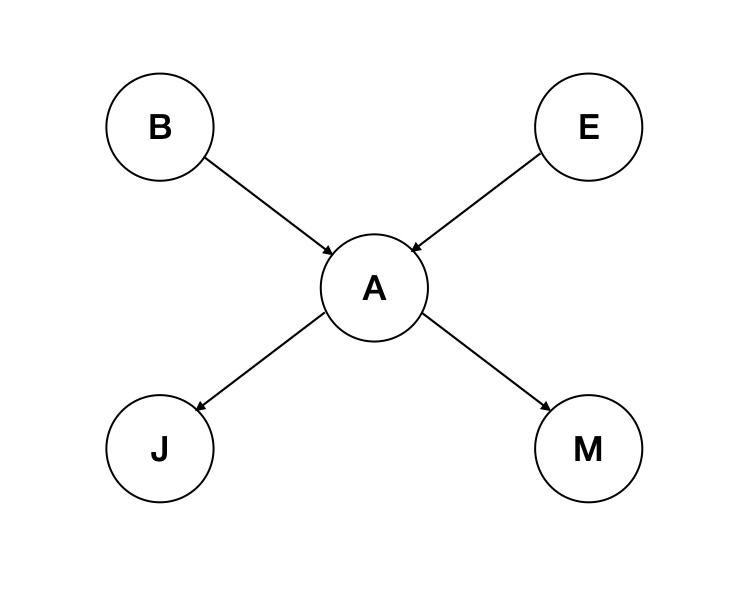
\includegraphics[width=0.5\linewidth]{hw3-figure1.jpg}
  \caption{第三题的贝叶斯网络}
  \label{hw3-figure1}
\end{figure}

\begin{enumerate}
\item 根据给定的贝叶斯网络对联合概率$P(B,E,A,J,M)$进行因子分解。

\item 对于变量$B$而言,我们给定哪一个或者两个变量的值,能够使得该变量条件独立于贝叶斯网络中的其他变量?

\item 如果我们给定变量$A$的值,其他的变量$(B,E,J,M)$之间有哪些是条件独立的?如果我们不给定变量$A$的值呢?注意,贝叶斯网络间两个节点条件独立可以写为$X_i \perp  X_j$。

\item 我们希望求解贝叶斯网络中$J=j, M=m, B=b$的概率,即$P(B=b_0, J=j_0, M=m_0)$。请根据联合概率的表达式列出计算$P(B=b_0, J=j_0, M=m_0)$的表达式。除此以外,请列出使用消元法求解$P(B=b_0, J=j_0, M=m_0)$的过程。为了方便,我们要求消元的顺序是$M\rightarrow J\rightarrow A\rightarrow E\rightarrow B$。
\end{enumerate}
\end{problem}

\begin{solution}
    \begin{enumerate}
        \item \begin{equation*}
            P(B,E,A,J,M) = P(J|A)P(M|A)P(A|B,E)P(B)P(E)
        \end{equation*}
        \item 给定其马尔科夫毯,即 $A,E$。
        \item 给定 $A$ 的值,$B\perp M,B\perp J,E\perp J,E\perp M,J\perp M$;不给定 $A$ 的值,$B\perp E$。
        \item 使用链式法则,
        \begin{align*}
            P(b,j,m) &= \sum_{e}\sum_a P(b,j,m,e,a) \\
            &= \sum_{e}\sum_{a} P(j|a)P(m|a)P(a|b,e)P(b)P(e) \\
            &= P(b)\sum_{e}P(e)\sum_{a}P(j|a)P(m|a)P(a|b,e)
        \end{align*}
        消元法求解:
        \begin{align*}
            &= \mathbf{f}_1(B)\times\sum_e \mathbf{f}_2(E)\times\sum_a \mathbf{f}_3(A|B,E)\times\mathbf{f}_4(A)\times\mathbf{f}_5(A) \\
            &= \mathbf{f}_1(B)\times\sum_e \mathbf{f}_2(E)\times\mathbf{f}_6(B,E) \\
            &= \mathbf{f}_1(B)\times\mathbf{f}_7(B)
        \end{align*}
        其中
        \begin{align*}
            \mathbf{f}_1(B) &=P(b)\\
            \mathbf{f}_2(E) &=\begin{pmatrix}
                P(e)\\
                P(\neg e)
            \end{pmatrix}\\
            \mathbf{f}_3(A|B,E) &= (P(a|b,e)\cdots P(\neg a|b,\neg e))_{2\times 1 \times 2} \\
            \mathbf{f}_4(A) &= \begin{pmatrix}
                P(j|a)\\
                P(j|\neg a)
            \end{pmatrix}\\
            \mathbf{f}_5(A) &= \begin{pmatrix}
                P(m|a)\\
                P(m|\neg a)
            \end{pmatrix}\\
            \mathbf{f}_6(B,E) &= \sum_a \mathbf{f}_3(A|B,E)\times\mathbf{f}_4(A)\times\mathbf{f}_5(A) = \mathbf{f}_3(a|B,E)\times\mathbf{f}_4(a) + \mathbf{f}_3(\neg a|B,E)\times\mathbf{f}_4(\neg a) \\
            \mathbf{f}_7(B) &= \sum_e \mathbf{f}_2(E)\times \mathbf{f}_6 (B,E) = \mathbf{f}_2(e)\times \mathbf{f}_6 (B,e) + \mathbf{f}_2(\neg e)\times \mathbf{f}_6 (B,\neg e)  
        \end{align*}
    \end{enumerate}
\end{solution}

%-------------------------------------------------------------
\begin{problem}
\indent 给定如下图\ref{hw3-figure3}所示的贝叶斯网络模型。我们希望从给定的模型中通过取样的方式进行一些概率的估算,且我们规定采样时该模型各节点的拓扑顺序为$(A\rightarrow B\rightarrow C\rightarrow D)。$\\
\begin{figure}[!htbp]
    \centering
    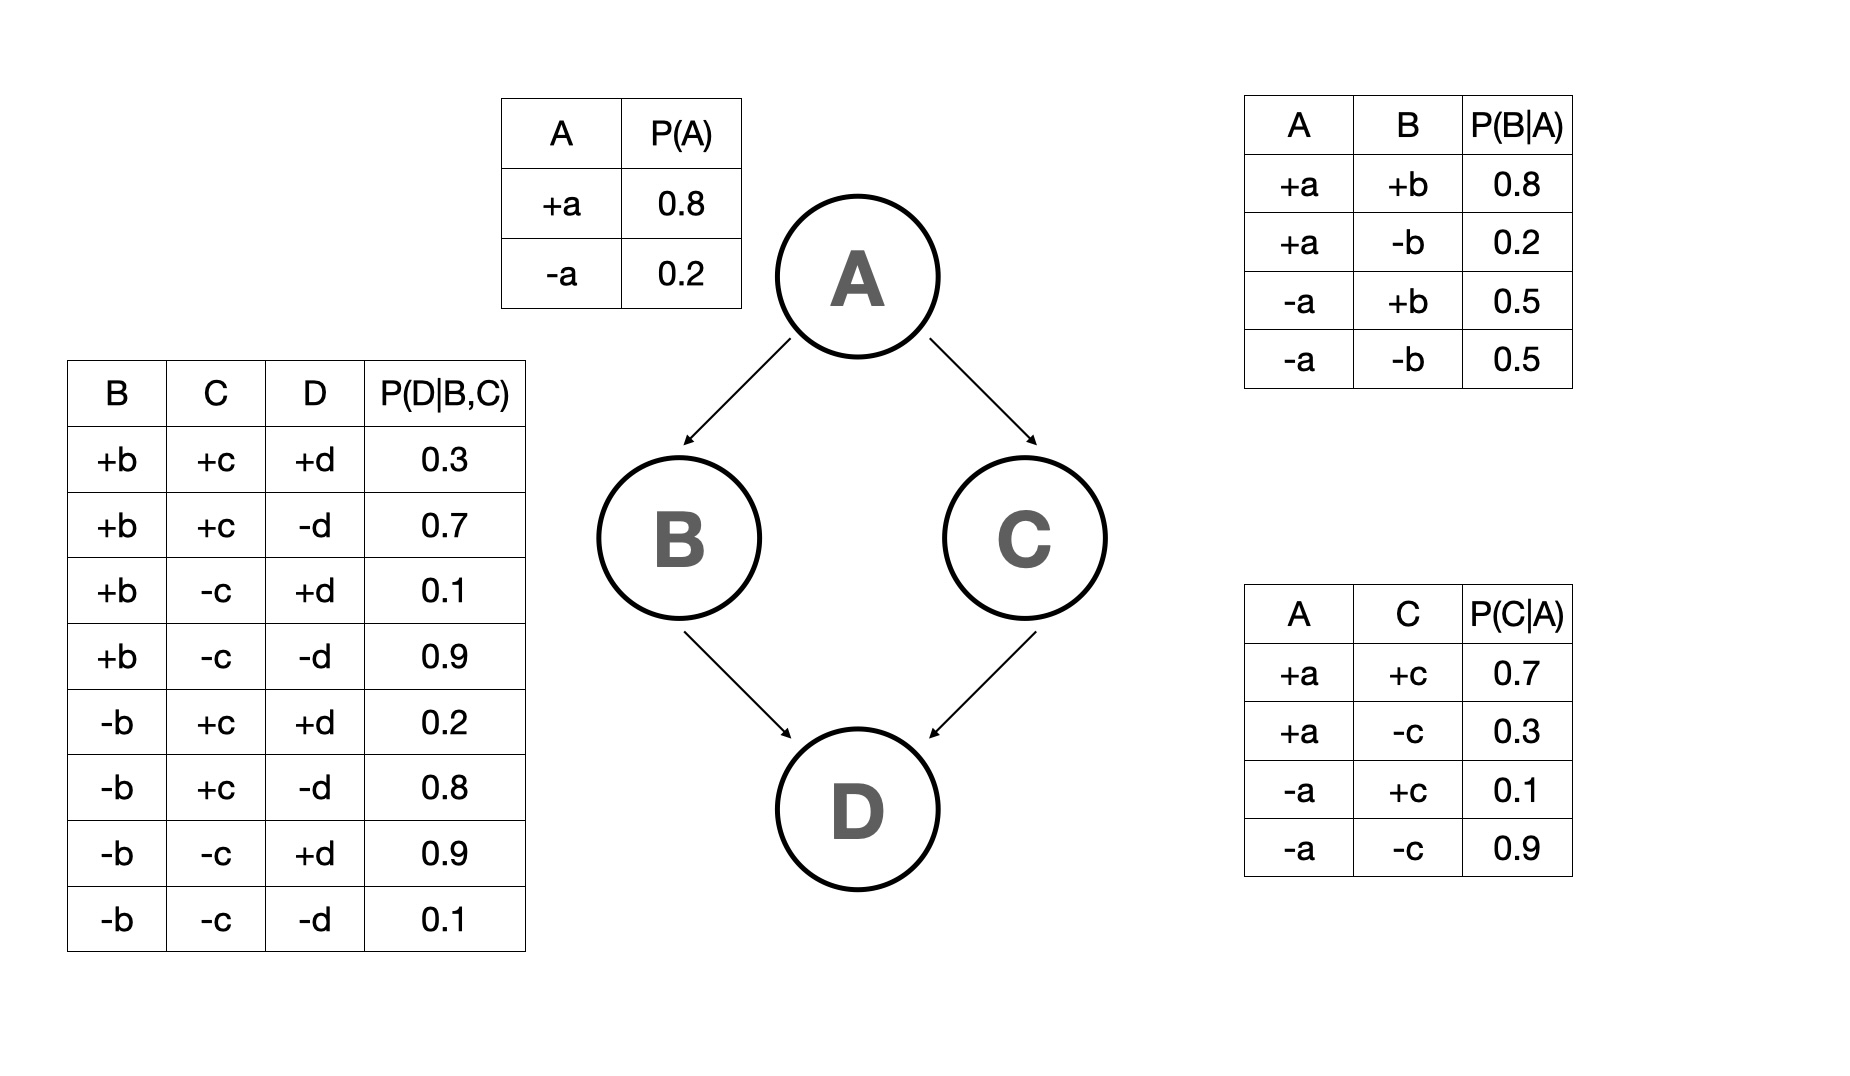
\includegraphics[width=1\linewidth]{hw3-figure3.jpg}
    \caption{第四题的贝叶斯网络}
    \label{hw3-figure3}
\end{figure}

\indent 示例:采用先验采样(prior sample)的方法生成样本。给定采样过程中的随机数为$(0.31\rightarrow 0.58\rightarrow 0.04 \rightarrow 0.94 \rightarrow 0.67 \rightarrow 0.49 \rightarrow 0.37 \rightarrow 0.42)$。
\begin{itemize}
    \item 首先我们取随机数$r=0.31$,而$r=0.31<P(+a)=0.8$,因此对于节点$A$我们取$+a$
    \item 接着随机数$r=0.58<P(+b|+a)=0.8$,因此对于节点$B$我们取$+b$
    \item 随机数$r=0.04<P(+c|+a)=0.7$,因此对于节点$B$我们取$+c$
    \item 随机数$r=0.94>P(+d|+b, +c)=0.3$,因此对于节点$D$我们取$-d$。这样我们通过一次采样得到了一个样本$(+a, +b, +c, -d)$
    \item 随机数$r=0.67<P(+a)=0.8$,因此对于节点$A$我们取$+a$
    \item 随机数$r=0.49<P(+b|+a)=0.8$,因此对于节点$B$我们取$+b$
    \item 随机数$r=0.37<P(+c|+a)=0.7$,因此对于节点$C$我们取$+c$
    \item 随机数$r=0.42>P(+d|+b, +c)=0.3$,因此对于节点$D$我们取$-d$。这样我们通过一次取样获得了一个新的样本$(+a, +b, +c, -d)$
    \item 采用了八个随机数,进行了两次采样,得到了两个样本,均为$(+a, +b, +c, -d)$
\end{itemize}
\end{problem}

\begin{enumerate}
    \item 采用拒绝采样的方法(rejection sampling)计算$P(-d|-b)$,请参照模型上方的示例写出采样过程(包括最后进行了几次采样,得到了怎样的样本)。采样时的随机数为$(0.31\rightarrow 0.58\rightarrow 0.04 \rightarrow 0.94 \rightarrow 0.67 \rightarrow 0.49\rightarrow 0.37 \rightarrow 0.42)$,且规定当随机数$r<P(+a)$时采样$+a$,当$r\geq P(+a)$时采样$-a$,随机数用完以后即废弃、当所有随机数用完整个算法停止。
    \begin{solution}
        \begin{itemize}
            \item 随机数取$r=0.31<0.8$,因此对于节点$A$我们取$+a$。
            \item 随机数取$r=0.58<P(+b|+a)=0.8$,因此对于节点$B$我们取$+b$。
            \item 随机数取$r=0.04<P(+c|+a)=0.7$,因此对于节点$C$我们取$+c$。
            \item 随机数取$r=0.94>P(+d|+b,+c)=0.3$,因此对于节点$D$我们取$-d$。\\
            本次采样的结果被丢弃,因为与证据$-b$不符合。
            \item 随机数$r=0.67<P(+a)=0.8$,因此对于节点$A$我们取$+a$。
            \item 随机数$r=0.49<P(+b|+a)=0.8$,因此对于节点$B$我们取$+b$。
            \item 随机数$r=0.37<P(+c|+a)=0.7$,因此对于节点$C$我们取$+c$。
            \item 随机数$r=0.42>P(+d|+b, +c)=0.3$,因此对于节点$D$我们取$-d$。\\
            本次采样的结果被丢弃,因为与证据$-b$不符合。
            \item 采用了八个随机数,进行了两次采样,得到0个样本。
        \end{itemize}
    \end{solution}
    \item 采用似然采样的方法(likelihood weighting sampling)计算$P(-d|-b)$,请参照模型上方的示例写出采样过程(包括最后进行了几次采样,得到了怎样的样本)。采样时的随机数为$(0.31\rightarrow 0.58\rightarrow 0.04 \rightarrow 0.94 \rightarrow 0.67 \rightarrow 0.49)$,且规定当随机数$r<P(+a)$时采样$+a$,当$r\geq P(+a)$时采样$-a$,随机数用完以后即废弃、当所有随机数用完整个算法停止。
    \begin{solution}
        \begin{itemize}
            \item 权值$w$为1.0。$A$不是一个证据变量,随机数取$r=0.31<0.8$,因此对于节点$A$我们取$+a$。
            \item $B$是一个证据变量,其值为 false,因此我们设置
            \begin{equation*}
                w\leftarrow w\times P(-b|+a) = 0.2
            \end{equation*}
            \item $C$不是一个证据变量,随机数取$r=0.58<0.7=P(+c|+a)$,因此对于节点$C$我们取$+c$。
            \item $D$不是一个证据变量,随机数取$r=0.04<0.2=P(+d| -b,+c)$,因此对于节点$D$我们取$+d$。\\
            事件[true, false, true, true]以权值0.2被记录到$D=-d$中去。
            \item 权值$w$为1.0。$A$不是一个证据变量,随机数取$r=0.94>0.8$,因此对于节点$A$我们取$-a$。
            \item $B$是一个证据变量,其值为 false,因此我们设置
            \begin{equation*}
                w\leftarrow w\times P(-b|-a) = 0.5
            \end{equation*}
            \item $C$不是一个证据变量,随机数取$r=0.67>0.1=P(+c|-a)$,因此对于节点$C$我们取$-c$。
            \item $D$不是一个证据变量,随机数取$r=0.49<0.9=P(+d| -b,-c)$,因此对于节点$D$我们取$+d$。\\
            事件[false, false, false, true]以权值0.5被记录到$D=+d$中去。
            \item 采用了六个随机数,进行了两次采样,得到了2个样本(一个正样本、一个负样本),$P(-d|-b)=\alpha\langle0.2,0.5\rangle=\langle 0.286, 0.714\rangle$。
        \end{itemize}
    \end{solution}
    \item 采用吉布斯采样的方法(Gibbs sampling)计算$P(-d|-b)$,请参照模型上方的示例写出采样过程(包括最后进行了几次采样,得到了怎样的样本)。采样时的随机数为$(0.31\rightarrow 0.58\rightarrow 0.04 \rightarrow 0.94 \rightarrow 0.67 \rightarrow 0.49)$,采样初时刻的节点取值初始化为$(+a, -b, +c, +d)$,且规定当随机数$r<P(+a)$时采样$+a$,当$r\geq P(+a)$时采样$-a$,随机数用完以后即废弃、当所有随机数用完整个算法停止。
    \begin{solution}
        \begin{itemize}
            固定$B=-b$,其余变量已经被初始化为$(+a,-b,+c,+d)$。
            \item 对$A$采样,$P(A| -b,+c)=\alpha P(A)P(-b|A)P(+c|A)=\alpha\langle 0.8\times 0.2\times 0.7, 0.2\times 0.5\times 0.1 \rangle=\alpha\langle 0.112, 0.01\rangle=\langle 0.918,0.082\rangle$,随机数$r=0.31<0.918=P(+a|-b,+c)$,所以$A$取$+a$。
            \item 对$C$采样,$P(C| +a,-b,+d)=\alpha P(C|+a)P(+d|-b,C)=\alpha\langle 0.7\times 0.2, 0.3\times 0.9 \rangle=\alpha\langle 0.14,0.27 \rangle=\langle 0.58,0.42\rangle$,随机数$r=0.58>0.341$,所以$C$取$-c$。
            \item 对$D$采样,$P(D| -b,-c)=\langle 0.9,0.1 \rangle$,随机数 $r=0.04<0.9=P(+d|-b,-c)$,所以$D$取$+d$。
            \item 本次采样的结果为 $(+a,-b,-c,+d)$。
            \item 对$A$采样,随机数$r=0.94>0.918=P(+a|-b,+c)$,所以$A$取$-a$。
            \item 对$C$采样,$P(C| -a,-b,+d)=\alpha P(C|-a)P(+d|-b,C)=\langle 0.1\times 0.2, 0.9\times 0.9\rangle=\langle 0.02,0.81 \rangle=\langle 0.024,0.976 \rangle$,随机数$r=0.67>P(+c|-a,-b,+d)=0.024$,所以$C$取$-c$。
            \item 对$D$采样,随机数$r=0.49<0.9=P(D|-b,-c)$,所以$D$取$+d$。
            \item 本次采样结果为 $(-a,-b,-c,+d)$。
            \item 采用六个随机数,进行了两次采样,得到了2个样本:$(+a,-b,-c,+d), (-a, -b, -c, +d)$ 皆为负样本。
        \end{itemize}
    \end{solution}
\end{enumerate}

%-------------------------------------------------------------
\begin{problem}
\indent 给定一个隐马尔可夫模型(HMM)。
\begin{enumerate}
    \item 运用HMM的建模方式,用条件概率的计算方式推导并化简$P(x_1,...,x_t,y_{t-1}=s_v,y_t=s_j)$。\\
\indent 提示:一般来说,我们会对HMM模型有以下的建模方式(与课件上一致)——$x_t$表示$t$时刻的观察状态,$y_t$表示$t$时刻的隐藏状态,隐藏状态可能取值为$\{1,2,3,\cdots, M \}$。初始状态的概率(start probabilities)表示为$\{ \pi_1, \cdots, \pi_M\}$,隐藏状态之间从状态$i$转化为状态$j$的转移概率(transition probabilities)为$a_{i,j}$,隐藏状态$y_i=s_j$与观察状态$x_i$之间的发散概率(emission probabilities)为$b_j(x_i)$。在使用前向算法推导序列概率的时候,设定的前向因子$ \alpha_t^i=P(x_1,...,x_t,y_t=s_i)$。
\begin{solution}
    \begin{align*}
        &P(x_1,...,x_t,y_{t-1}=s_v,y_t=s_j) \\
        =& \sum_{y_1}\sum_{y_2}\cdots\sum_{y_{t-2}}\pi_{y_1}\times\prod_{\tau=2}^{t-2}a_{y_\tau,y_{\tau+1}}\times\prod_{\tau=1}^{t-2} P(x_\tau|y_\tau)\times a_{t-1,t} P(x_{t-1}|y_{t-1}=s_v) P(x_t|y_t=s_j)\\
        =& a_{y_t-1=s_v,y_t=s_j} P(x_{t-1}|y_{t-1}=s_v) P(x_t|y_t=s_j) \sum_{i=1}^M\alpha_{t-2}^i\\
        =& a_{y_t-1=s_v,y_t=s_j} b_{v}(x_{t-1})b_{j}(x_t)\sum_{i=1}^M\alpha_{t-2}^i
    \end{align*}
    其中
    \begin{equation*}
        \alpha_\tau^i = b_{i}(x_{\tau})\sum_{k=1}^M \alpha_{\tau-1}^k a_{k,i}
    \end{equation*}
\end{solution}
    \item 我们给定的HMM模型如下图\ref{hw3-figure2}所示。假定图中的圆圈表示$A, B, C$三种可能的隐藏状态,而圆圈中的数字表示特定隐藏状态下的观察状态以及其发射概率(emission probabilities)。圆圈之间的箭头表示隐藏状态的转移以及相应的转移概率(transition probabilities)。我们用$p_{y=A}^t$表示在$t$时刻,隐状态为$A$的概率,用$p_{x=1}^t$表示在$t$时刻,观察状态为$1$的概率。为了简便,我们规定初始的隐状态为$A$,即$p_A^1 = 1$。在每个时刻,隐状态会通过转移概率确定下个时刻的状态。\\
\indent (a)请用图中给定的数值与符号计算$p_{y=C}^3$。\\
\indent (b)假设在$t$时刻,$(p_{y=B}^t, p_{y=C}^t)$分别为$(b_0, c_0)$,请用图中给定的数值与符号计算$p_{x=2}^t$。
\begin{figure}[h]
    \centering
    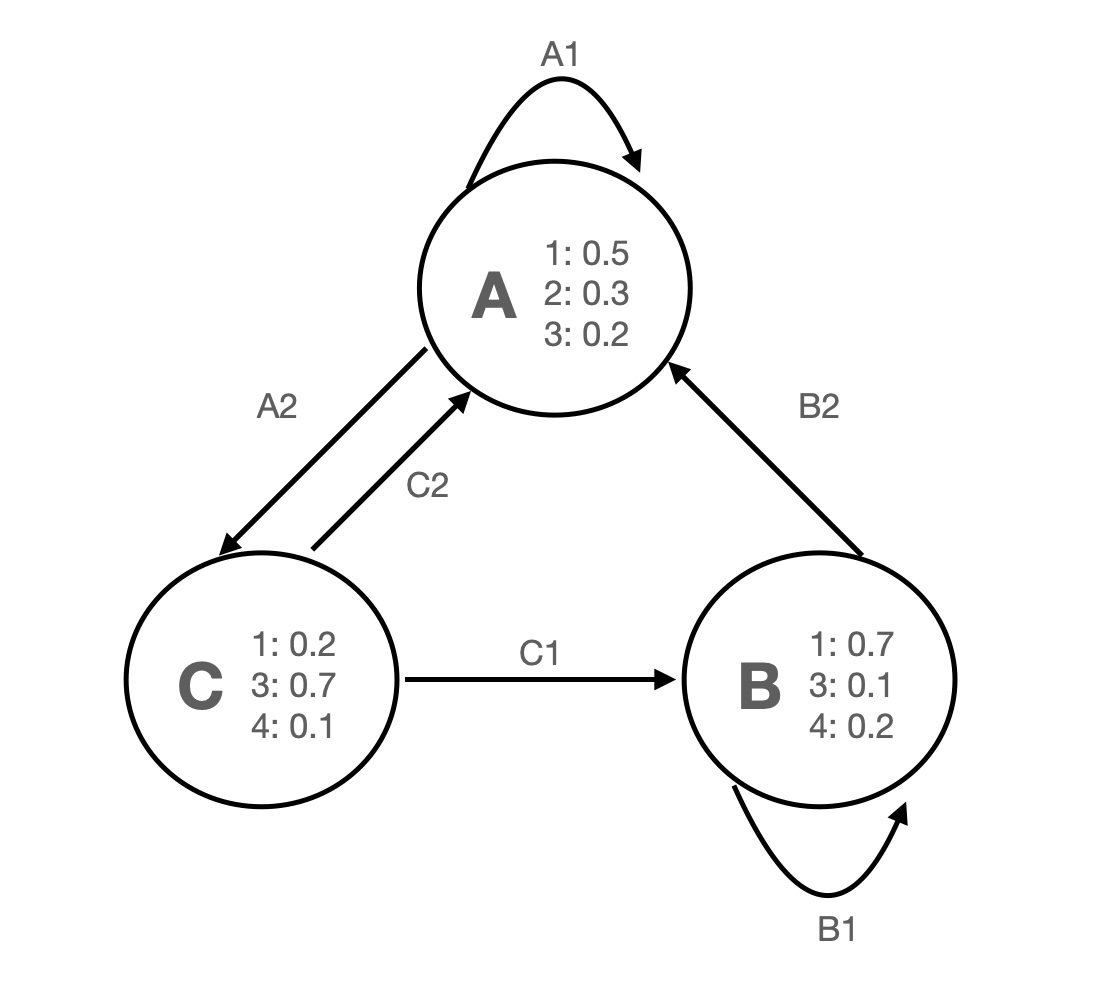
\includegraphics[width=0.8\linewidth]{hw3-figure2.jpg}
    \caption{第四题第二小问的HMM模型}
    \label{hw3-figure2}
\end{figure}
\begin{solution}
    \begin{enumerate}
        \item[(a)] 由于没有给定观察状态,所以
        \begin{align*}
            p_{y=C}^3 =& \sum_{y_1}\sum_{y_2} P(y_1)P(y_2|y_1)P(y_3=C|y_2)\\ 
            =& \sum_{y=2} P(y_2|y_1=A)P(y_3=C|y_2)\\
            =& P(y_2=A|y_1=A)P(y_3=C|y_2=A)+P(y_2=C|y_1=A)P(y_3=C|y_2=C)\\
            =& A_1 A_2 + A_2 \times 0\\
            =& A_1 A_2
        \end{align*}
        \item[(b)] 使用后向算法推算,其中$p_{y=A}^t=1-b_0-c_0$:
        \begin{align*}
            p_{x=2}^t =& \sum_{y=t}P(x_t=2,y_t)\\
            =& \sum_{y=t}P(y_t)P(x_t=2|y_t)\\
            =& P(y_t=A)P(x_t=2,y_t=A) + P(y_t=B)P(x_t=2,y_t=B) \\&+ P(y_t=C)P(x_t=2,y_t=C)\\
            =& 0.3(1-b_0-c_0)
        \end{align*} 
    \end{enumerate}
\end{solution}
\end{enumerate}
\end{problem}

\end{document}